\section{Specific Requirement}

\subsection{External Interface Requirements}
\textbf{SafeStreets} is a mobile based application, the following section will give a more detailed description, in terms of hardware, software and communication interfaces.
\subsubsection{User Interfaces}
    \textbf{Login} \newline When a Guest downloads SafeStreets for the first time, the first interface will be the login one. In \textit{Figure 4} it is also shown that if the Guest doesn't have an account it is possible to proceed by registering and creating a new account.\vspace{1cm}
    \begin{figure}[h]
        \centering
        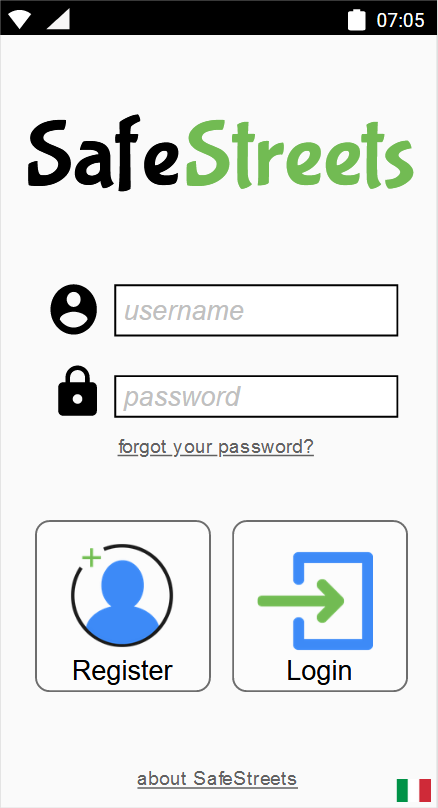
\includegraphics[scale=0.7]{Images/login.png}
        \caption{Login interface}
    \end{figure}\newpage
    \noindent\textbf{Register}\newline
    In the register interface \textit{Figure 5}. It will be asked to the Guest to insert his/her personal information, to upload an Identification card (since it is required that all accounts must be authenticated) and to choose an \textit{Username} and a \textit{Password}.
        \begin{figure}[h]
        \centering
        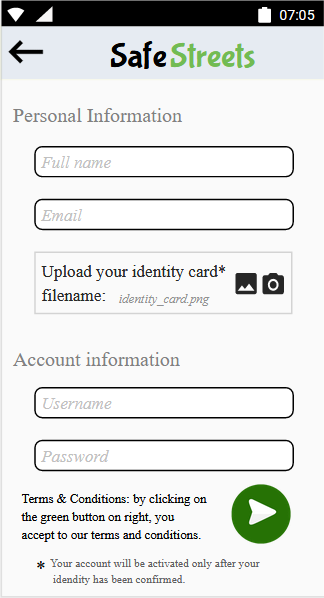
\includegraphics[scale=0.89]{Images/register.png}
        \caption{Register interface}
    \end{figure}
    \newline\textbf{User Home Page}\newline
    This activity contains all the possible functionalities that a simple User can use. Thus, a User can:
    \begin{itemize}
        \item Report a Traffic Violation.
        \item View his/her own notifications sent to Authorities and their status.
        \item View statistics like the effectiveness of the application, the most egregious offenders, etc.
        \item Open a Map that shows safe and unsafe areas (with the option to use also the data from municipality).
    \end{itemize}
    \begin{figure}[h]
    \centering
    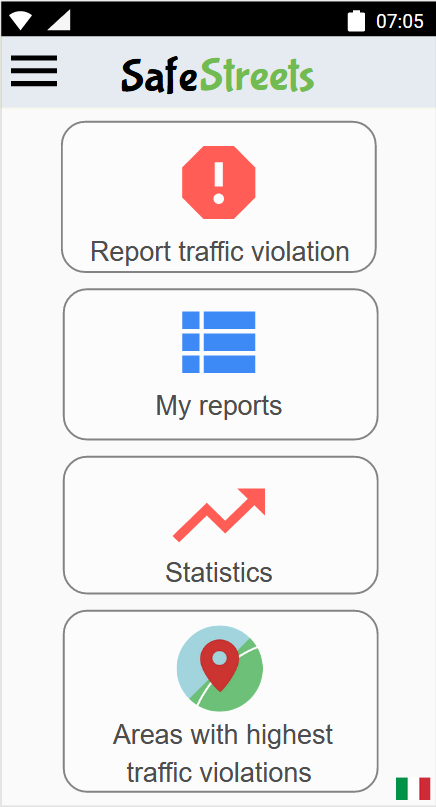
\includegraphics[scale=0.8]{Images/user_menu.png}
    \caption{User Home Page interface}
    \end{figure}\newpage
    \noindent\textbf{Authority Home Page}\newline
    For Authorities the functions available are a bit different, an authority can:
    \begin{itemize}
        \item Access to the notifications sent by users.
        \item View the traffic tickets generated.
        \item Get the suggestions elaborated by the application.
        \item View statistics like the effectiveness of the application, the most egregious offenders, etc.
        \item Open a Map that shows safe and unsafe areas (with the option to use also the data from municipality).
    \end{itemize}
    \begin{figure}[h]
    \centering
    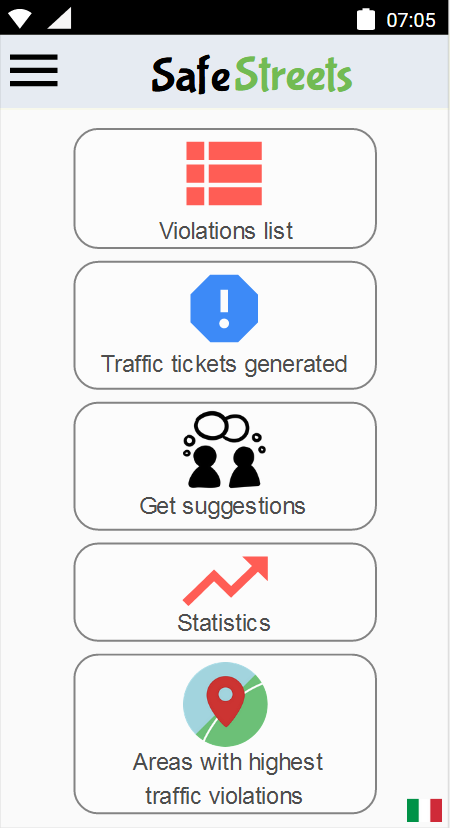
\includegraphics[scale=1]{Images/authority_menu.png}
    \caption{Authority Home Page interface}
    \end{figure}
    $          $\newline\\\\
    \textbf{Report a traffic violation}\newline
    This form allows users to notify authorities when traffic violations occur, an user takes a photo of the violation, selects the type of the violation and inserts the location where it occurred. Moreover, the User can also include further information about the vehicle like the license plate, the model, etc.
        \begin{figure}[h]
        \centering
        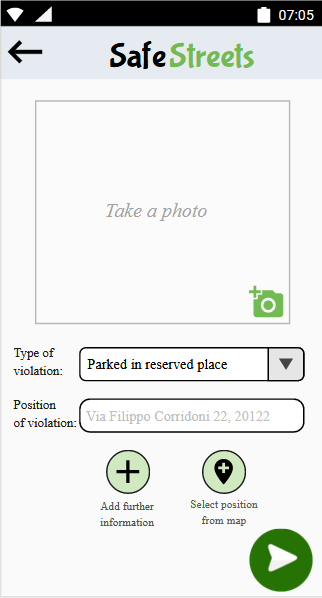
\includegraphics[scale=0.85]{Images/report_violation.png}
        \caption{Report traffic violation interface}
    \end{figure}
    \textbf{My Reports}\newline
    Once a User sent a notification it is possible to see all the notifications sent to authorities, \textit{Figure 9}. In this activity it is also possible to search them by their ID and see their status. There are three possible status: to be seen, accepted, rejected.
        \begin{figure}[h]
        \centering
        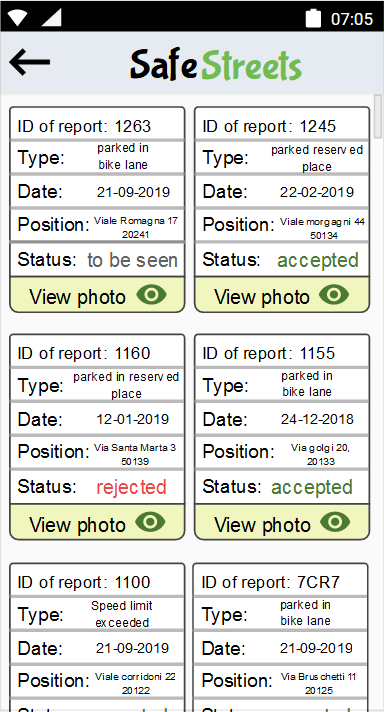
\includegraphics[scale=0.85]{Images/my_reports.png}
        \caption{My reports interface}
    \end{figure}\newpage
    \noindent\textbf{Violations list}\newline
    An Authority is able to see all the violations sent by users, the list shows the most important information to know if an Authority is interested or not in that violation; type, date and position. It is also possible to see the trustness of the User who sent each notification.\newline
            \begin{figure}[h]
        \centering
        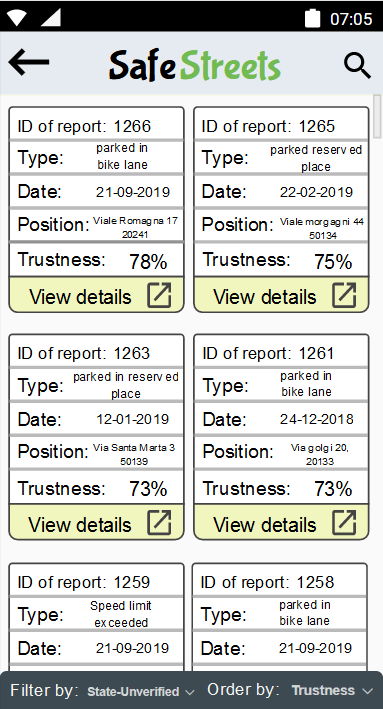
\includegraphics[scale=0.85]{Images/report_lists.png}
        \caption{Violations list interface}
    \end{figure}
    \newline
    \textbf{Details about a notification}\newline
    After an Authority clicks on \textit{View details} from the Violations list, he can access to details like license plate, model of the car, position where the violation occurred, the picture sent by the user, etc. The license plate of being shown is the output obtained from a image recognition algorithm, this output comes also with a number $\in [0,1]$ that represents the accuracy of the license plate obtained.
    \begin{figure}[h]
        \centering
        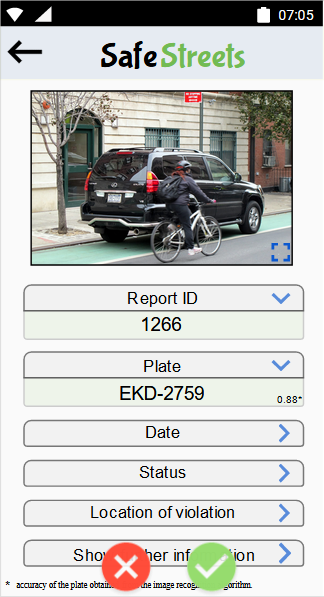
\includegraphics[scale=0.85]{Images/violation_info.png}
        \caption{Details about a report}
    \end{figure}\newline
    \textbf{Traffic tickets generated}\newline
    In the previous activity it was possible to see that an Authority can press on $X$ button to reject a report from a user or to press on the check button to accept and  generate a traffic ticket related to it. In \textit{Figure 12} all the traffic tickets generated by the Authority logged in are shown, It is possible to download the traffic ticket as a PDF file.
       \begin{figure}[h]
        \centering
        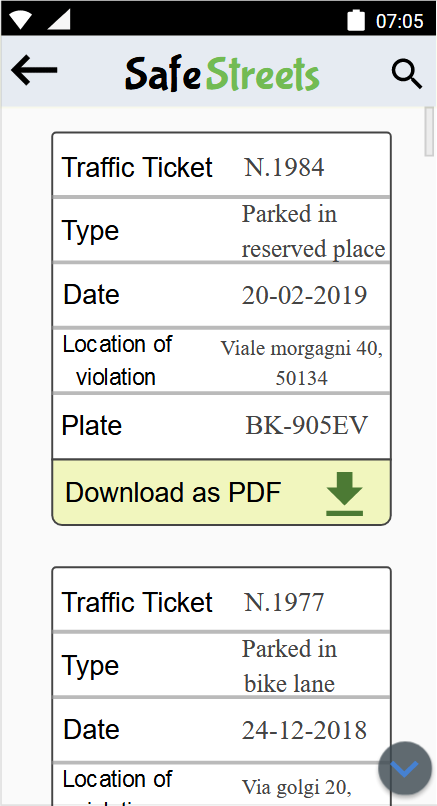
\includegraphics[scale=0.85]{Images/traffic_ticket.png}
        \caption{Traffic tickets interface}
    \end{figure}\newline
    \textbf{Get Suggestions}\newline
    \textit{Figure 13} shows the list of possible suggestions that authorities can see, each Authority see only the possible suggestions related to the own city, so this list can be shared between different districts but in the same city. An authority can print the suggestion by downloading as a PDF file or he/she can share it to the department in charge of receiving suggestions by citizens. The suggestions are taken from an AI algorithm  that is continuously updating its own dataset by modifying the effectiveness of each possible solution to each problem.  
    
       \begin{figure}[h]
        \centering
        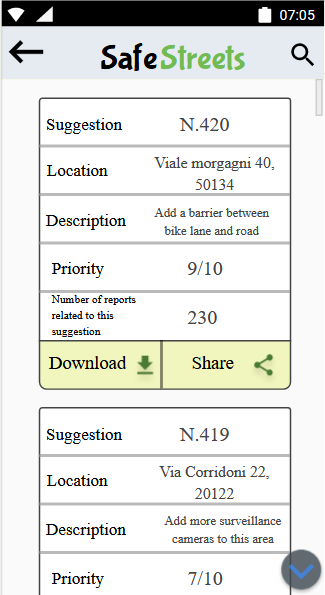
\includegraphics[scale=1]{Images/suggestions.png}
        \caption{Get suggestions interface}
    \end{figure}\newpage
    \noindent\textbf{Statistics}
    % non mi viene la parola, non influenzare ma c'era una parola bellina che non mi ricordo, not affecting né influencing
    Users and authorities can also see statistics about traffic violations and how SafeStreets is ... in streets safeness. An example is the graph \textit{Effectiveness of SafeStreets}, in this graph it is possible to see how the rate between traffic tickets generated and notifications sent has been increasing since the last years.  
       \begin{figure}[h]
        \centering
        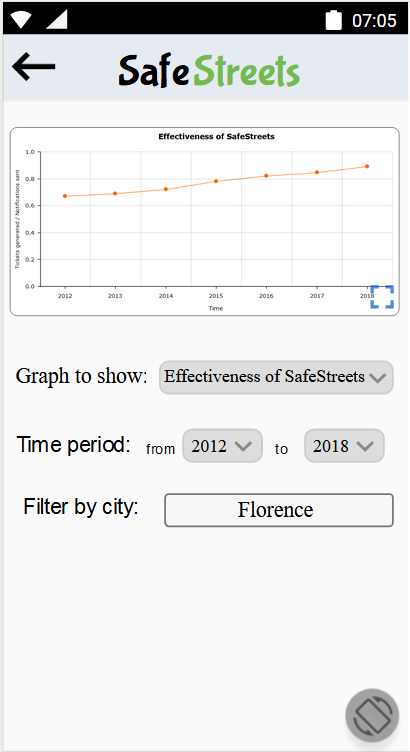
\includegraphics[scale=0.9]{Images/Statistics.png}
        \caption{Statistics interface}
    \end{figure}
    \newline\textbf{Areas with highest traffic violations}\newline
    This activity gives the possibility to see the tag assigned to each area in which SafeStreets has been used (or areas that are present in a service offered by the municipality). There are 4 possible labels: Safe, unsafe, Very safe and dangerous. The tags inferred can be produced by merging the own data of SafeStreets with the data retreived from a service provided by the Municipality, if the option is enabled.\newline 
       \begin{figure}[h]
        \centering
        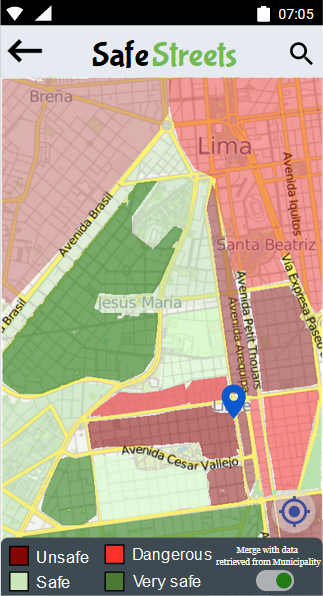
\includegraphics[scale=0.9]{Images/safe_unsafe.png}
        \caption{Safe/Unsafe areas interface}
    \end{figure}
    \newpage
\subsubsection{Hardware Interfaces}

\subsubsection{Software Interfaces}

\subsubsection{Communication Interfaces}

\subsection{Functional Requirements}
\subsubsection{Use Cases}


%%%%%%%%  use casessssss %%%%%%%%%%%%%%%%%%%%%%%


\begin{table}[ht]
\begin{tabular}{|l|p{0.9\textwidth}|}
\hline
\textbf{ID}             & UC1                                                                             \\ \hline
\textbf{Description}    & A \textit{Guest} creates a normal \textit{User} account to use the application \\ \hline
\textbf{Actors}         &   \textit{Guest}                                                                            \\ \hline

\textbf{Preconditions}  &   \begin{itemize}

 \item \textit{Guest} has downloaded the app onto his device
   \item      \textit{Guest} has a working internet connectivity
     \item       \textit{Guest} hasn't an account still.
                 \end{itemize}     
                    \\ \hline
                    
\textbf{Flow of Events} &   \begin{enumerate}
    \item The \textit{System} ask the \textit{Guest} to Log in or to Register
    \item The \textit{Guest} choose the Register option
    \item The \textit{System} return the registration form
    \item The \textit{Guest} fill in the form with its personal information and click confirm button
    \item The \textit{System} checks the validity of the input
    \item The \textit{System} generates a new account with a new identifier
    \item The \textit{System} sends a confirmation e-mail to the \textit{Guest}
\end{enumerate}                                                                             \\ \hline
\textbf{Postconditions} &  The \textit{Guest} becomes a \textit{User}, and is now able to log in and use the application services                                                                     \\ \hline

\textbf{Exceptions} &    \begin{itemize}
    \item The \textit{Guest} inputs a non-valid e-mail address
    \item The \textit{Guest} inputs a password that not matches with security standards. 
    \end{itemize} 
  In both cases, the \textit{System} will not let the confirm button to be pressed until all fields are correctly filled in.
                                                                            \\ \hline
\end{tabular}
\end{table}



%UC2




\begin{table}[ht]
\begin{tabular}{|l|p{0.9\textwidth}|}
\hline
\textbf{ID}             & UC2                                                                             \\ \hline
\textbf{Description}    & A normal \textit{User} logs in \\ \hline
\textbf{Actors}         &   \textit{User}                                                                            \\ \hline

\textbf{Preconditions}  &   \begin{itemize}

 \item \textit{User} has downloaded the app onto his device
   \item      \textit{User} has a working internet connectivity
     \item       \textit{User} has an account
                 \end{itemize}     
                    \\ \hline
                    
\textbf{Flow of Events} &   \begin{enumerate}
    \item The \textit{System} ask the \textit{User} to Log in or to Register
    \item The \textit{User} choose the log in option
    \item The \textit{System} return the log in form
    \item The \textit{User} fill in the form with its log in data, and press the log in button
    \item The \textit{System} checks the validity and the matching of the inputs
    \item The \textit{User} accesses the interface with the various \textit{User} functions

\end{enumerate}                                                                             \\ \hline
\textbf{Postconditions} &  The \textit{User} is now able  to browse in the application and to use the application services                                                                     \\ \hline

\textbf{Exceptions} &    \begin{itemize}
    \item The \textit{User} inputs a non-existing username
    \item The \textit{User} inputs a wrong password for that username. 

\end{itemize}                                             The flow of the events restarts at point 4, showing an error message.                                \\ \hline

\end{tabular}
\end{table}


%UC3




\begin{table}[ht]
\begin{tabular}{|l|p{0.9\textwidth}|}
\hline
\textbf{ID}             & UC3                                                                             \\ \hline
\textbf{Description}    & A normal \textit{User} notifies a violation \\ \hline
\textbf{Actors}         &  \textit{User, System}                                                                       \\ \hline

\textbf{Preconditions}  &   \begin{itemize}

 \item \textit{User} is logged in the application
                 \end{itemize}     
                    \\ \hline
                    
\textbf{Flow of Events} &   \begin{enumerate}
    \item The \textit{User} browse to the report violation section
    \item The \textit{System} return the form for reporting a violation
    \item The \textit{User} fill in the form with the mandatory data
    \item The \textit{User} press the button to take a picture of the violation
    \item The \textit{User} press the send button, and send the notification.
    \item The \textit{System} runs an algorithm to extract metadata about the notification, and to check the validity of the information. Then submits the report to the \textit{Authorities}.
    \item The \textit{System} add the report to the \textit{User} reports section. 

\end{enumerate}                                                                             \\ \hline
\textbf{Postconditions} & \begin{itemize}
     
 \item The \textit{User} can see the his/her new report and its status in the \textit{My Report} section. 
 
 \item The Authorities can see the notification in their report list
 \end{itemize}\\ \hline

\textbf{Exceptions} &    \begin{itemize}
    \item The \textit{User} inputs non valid data
    \item The \textit{User} doesn't input some mandatory data.

\end{itemize}
The send button will not be available until fields are correctly filled in.

\begin{itemize}
    \item The \textit{System} will find irregularities by running its algorithms.
\end{itemize}
In this case, the notification will be rejected.     
                           \\ \hline

\end{tabular}
\end{table}





%%%%%%%%%%%%%% fine use casesss %%%%%%%%%%%%%5


    \subsubsection{Sequence Diagrams}
    
    \begin{figure}[h]
        \centering
        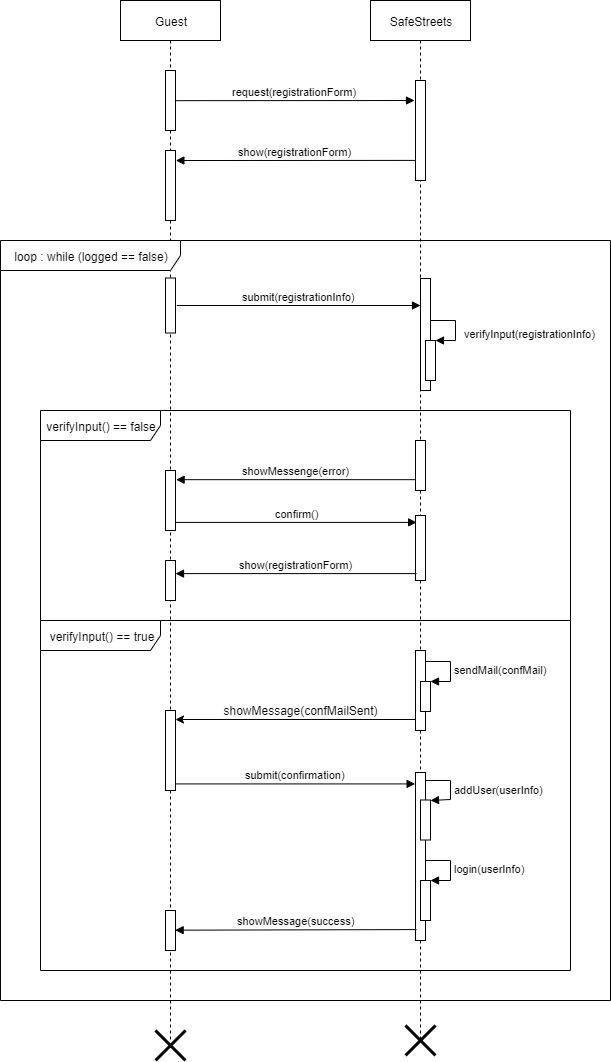
\includegraphics[scale=0.5]{Images/SeqDiag_registration.png}
        \caption{Sequence Diagram of the registration of a User}
    \end{figure}
    
    \begin{figure}[h]
        \centering
        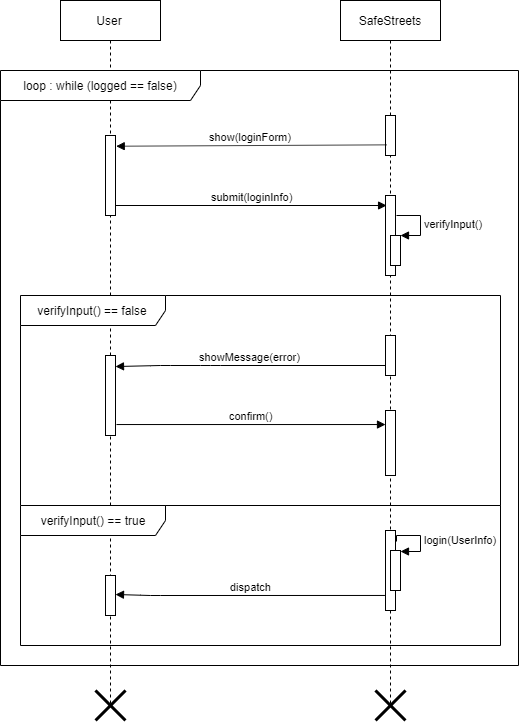
\includegraphics[scale=0.5]{Images/SeqDiag_login.png}
        \caption{Sequence Diagram of the login of a User or of an Authority}
    \end{figure}
    
    \begin{figure}[h]
        \centering
        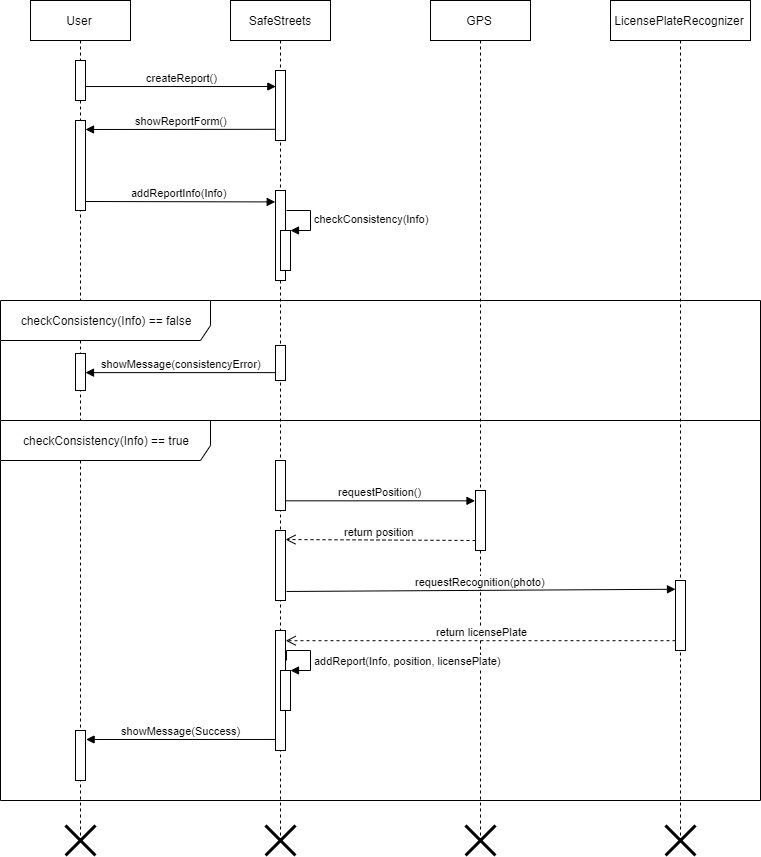
\includegraphics[scale=0.5]{Images/SeqDiag_addReport.png}
        \caption{Sequence Diagram of the insertion of a Report by a User}
    \end{figure}
    
    \begin{figure}[h]
        \centering
        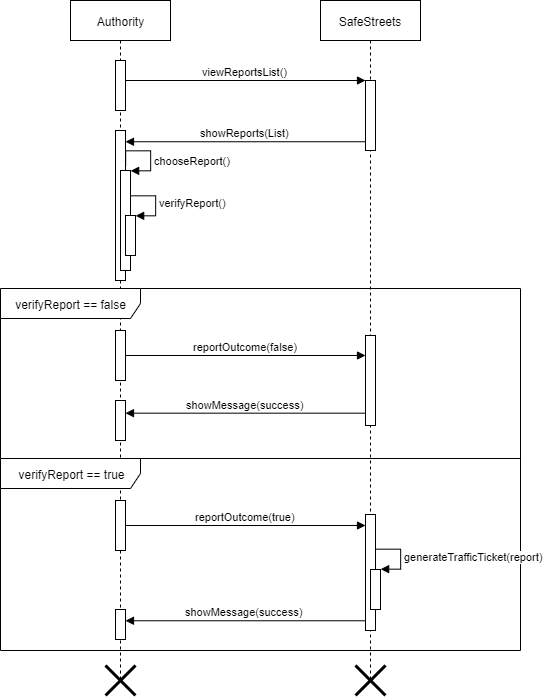
\includegraphics[scale=0.5]{Images/SeqDiag_generateTrafficTicket.png}
        \caption{Sequence Diagram of the checking of a Report and, eventually, the generation of the corresponding Traffic Ticket}
    \end{figure}
    
    \begin{figure}[h]
        \centering
        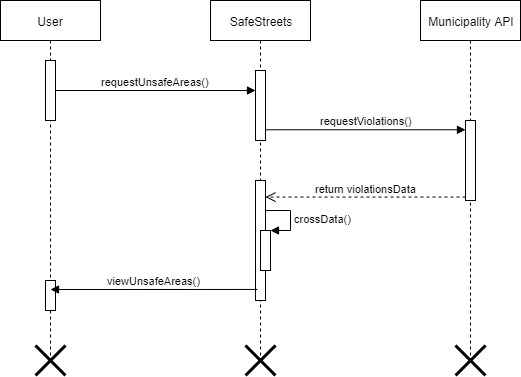
\includegraphics[scale=0.5]{Images/SeqDiag_unsafeAreas.png}
        \caption{Sequence Diagram of the request to know which are the unsafe areas}
   \end{figure}

\subsection{Performance Requirements}

\subsection{Design
Constraints}

\subsubsection{Standards compliance}

\subsubsection{Hardware
limitations}

\subsubsection{Any other constraint}

\subsection{Software System Attributes}

\subsubsection{Reliability}

\subsubsection{Availability}

\subsubsection{Security}

\subsubsection{Maintainability}

\subsubsection{Portability}
